\documentclass[11pt]{article}
\usepackage[english]{babel}
\usepackage{natbib}
\usepackage{url}
\usepackage[utf8x]{inputenc}
\usepackage{amsmath}
\usepackage{graphicx}
\graphicspath{{images/}}
\usepackage{parskip}
\usepackage{fancyhdr}
\usepackage{vmargin}
\setcitestyle{square}
\setmarginsrb{3 cm}{2.5 cm}{3 cm}{2.5 cm}{1 cm}{0.75 cm}{1 cm}{1.5 cm}
\usepackage[justification=centering]{caption}
\title{A survey on Soil-Water Sensors in the Agriculture Sector}								% Title
										% Date

\makeatletter
\let\thetitle\@title
\let\theauthor\@author
\let\thedate\@date
\makeatother

\pagestyle{fancy}
\fancyhf{}
\rhead{\theauthor}
\lhead{\thetitle}
\cfoot{\thepage}

\begin{document}

%%%%%%%%%%%%%%%%%%%%%%%%%%%%%%%%%%%%%%%%%%%%%%%%%%%%%%%%%%%%%%%%%%%%%%%%%%%%%%%%%%%%%%%%%

\begin{titlepage}
	\centering
    \vspace*{0.5 cm}
    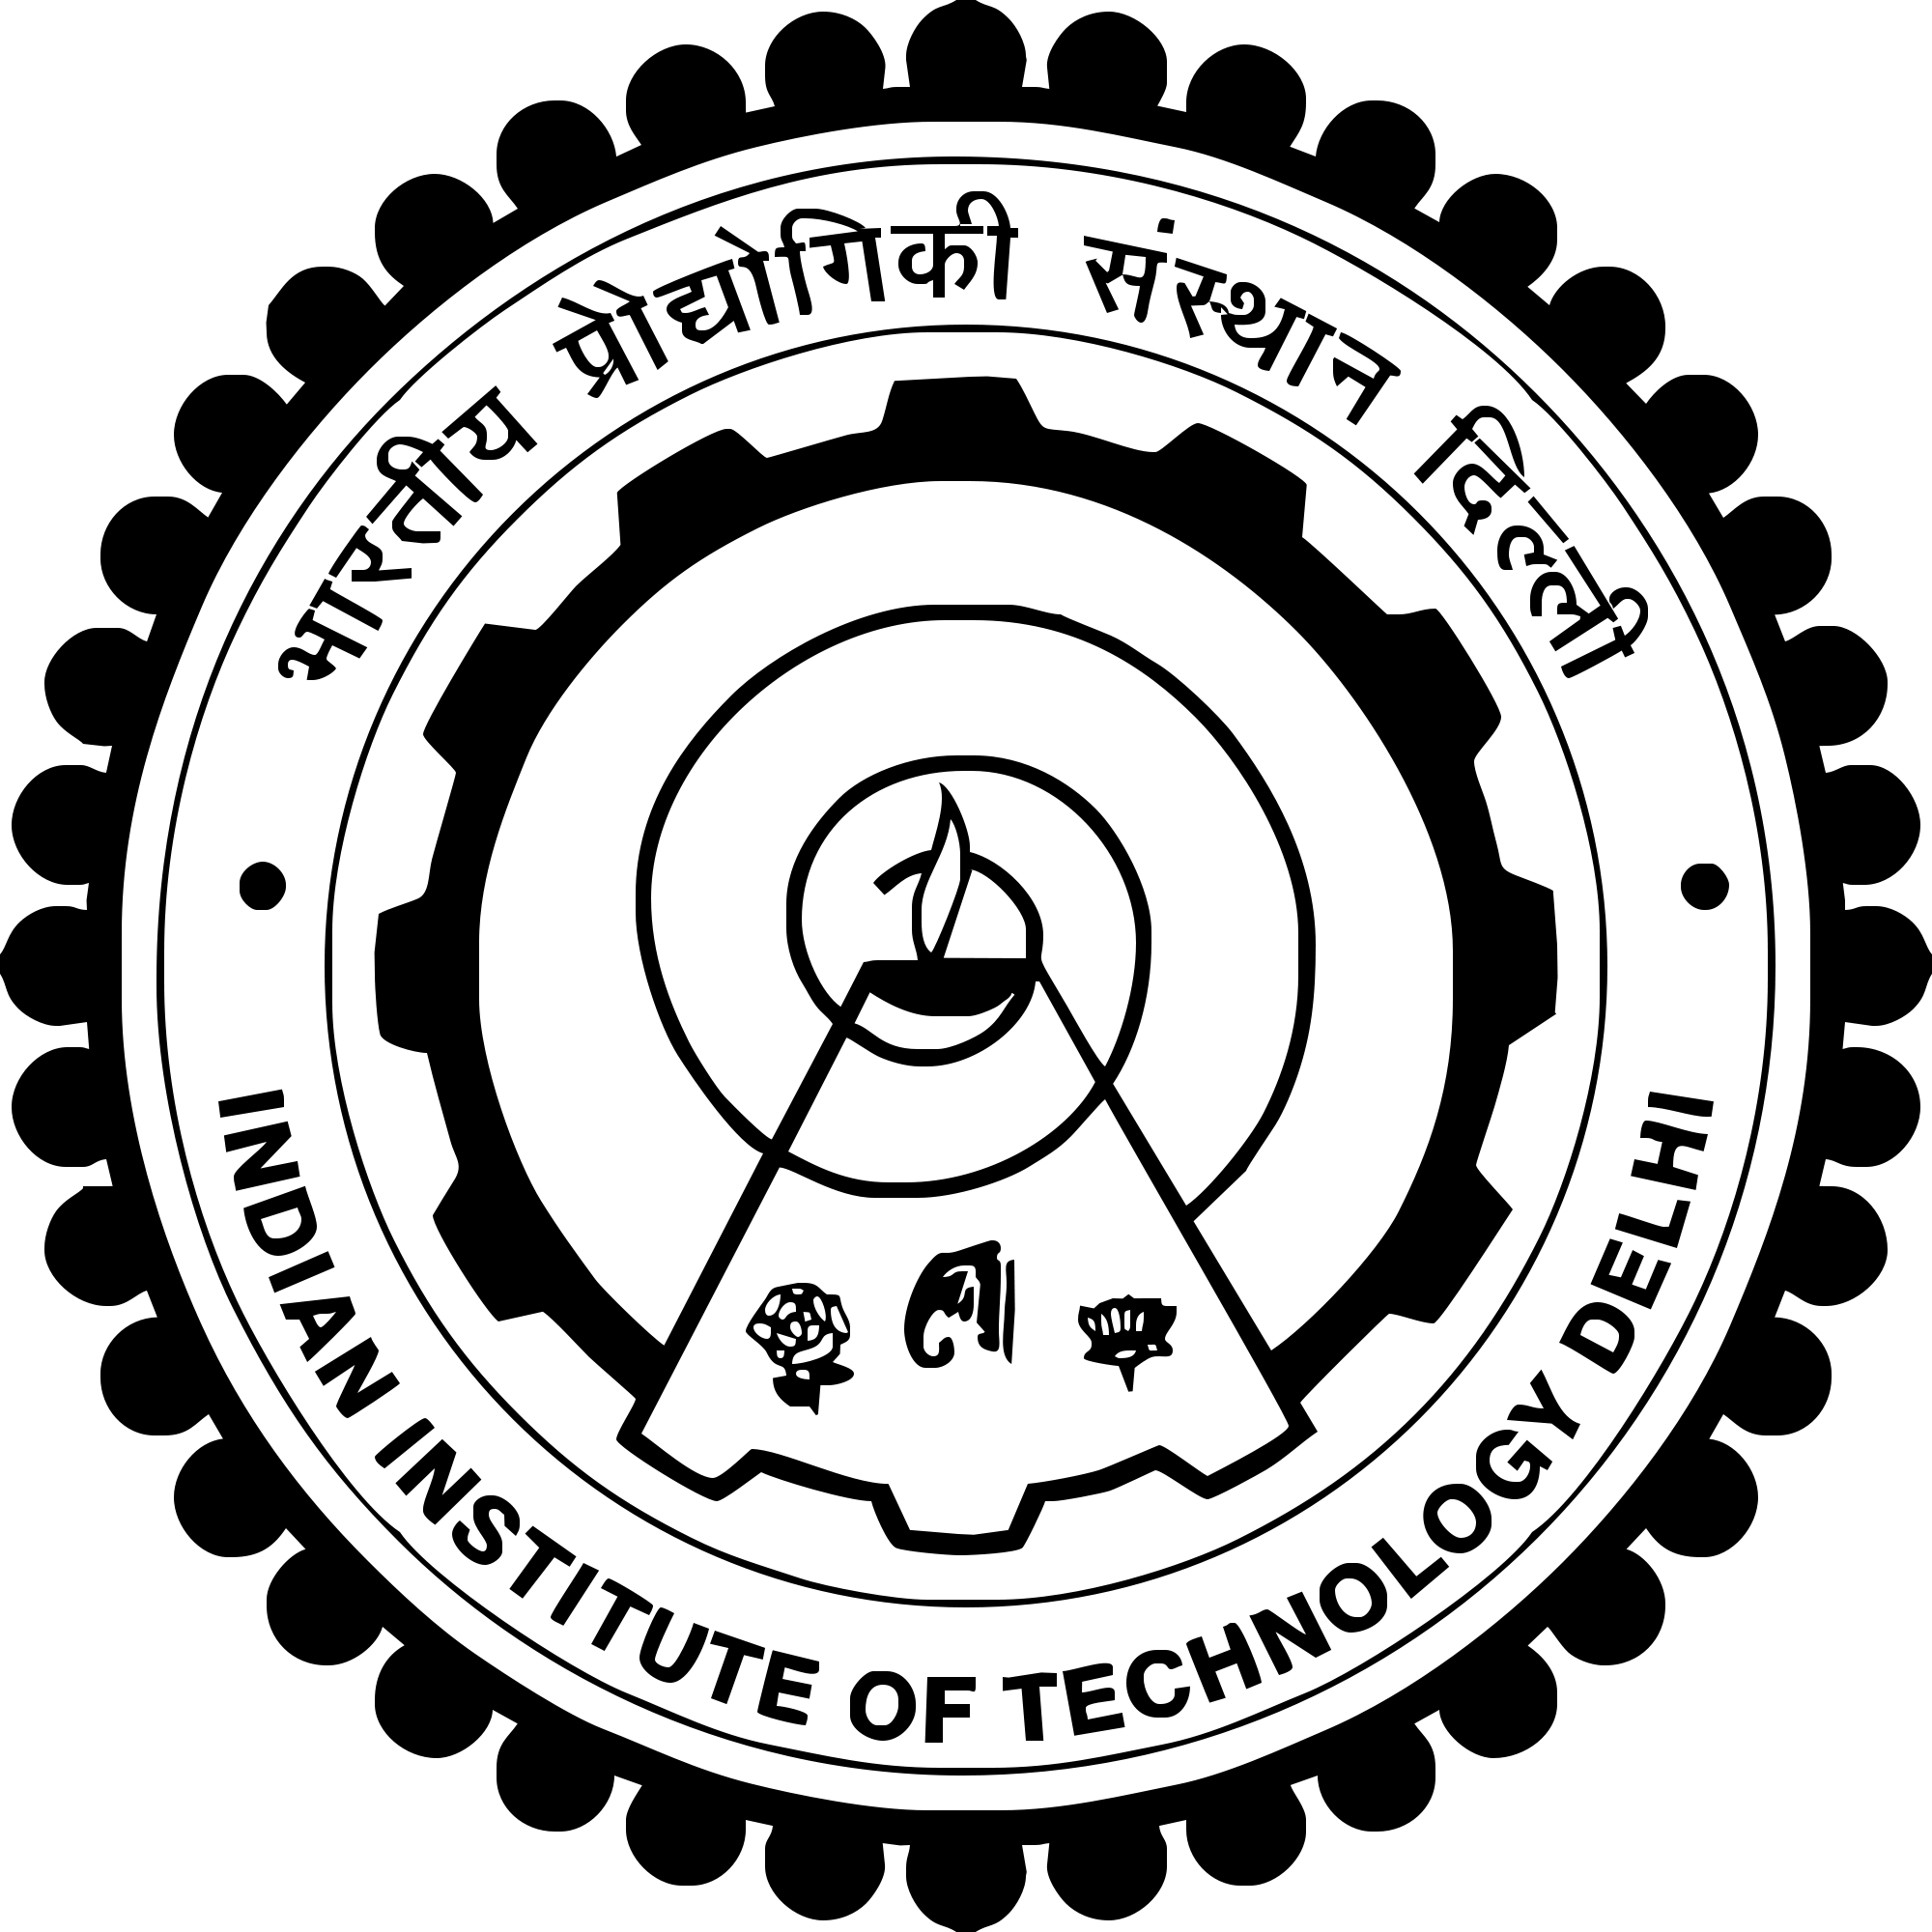
\includegraphics[scale = 0.075]{IIT_Delhi_logo.png}\\[1.0 cm]	% University Logo
    \textsc{\LARGE Indian Institute of Technology Delhi}\\[2.0 cm]	% University Name
	\textsc{\LARGE ELL301 Homework}\\[0.5 cm]				% Course Code
	\rule{\linewidth}{0.2 mm} \\[0.4 cm]
	{ \huge \bfseries \thetitle}\\
	\rule{\linewidth}{0.2 mm} \\[3.5 cm]
	
	\begin{minipage}{0.4\textwidth}
		\begin{flushleft} \large
			\emph{Submitted To:}\\
			Dr. Shaunak Sen\\
			Associate Professor\\
			Dept. of Electrical Engg\\
			IIT Delhi
			\end{flushleft}
			\end{minipage}~
			\begin{minipage}{0.4\textwidth}
            
			\begin{flushright} \large
			\emph{Submitted By :} \\
            Gantavya Bhatt\\
            2016EE10694\\
			Dept. of Electrical Engg\\
            IIT Delhi\\
            \texttt{ee1160694@ee.iitd.ac.in}
		\end{flushright}
        
	\end{minipage}\\[2 cm]
	
\end{titlepage}

%%%%%%%%%%%%%%%%%%%%%%%%%%%%%%%%%%%%%%%%%%%%%%%%%%%%%%%%%%%%%%%%%%%%%%%%%%%%%%%%%%%%%%%%%

\tableofcontents
\pagebreak
%figure1 ka reference-> https://www.researchgate.net/figure/Four-stroke-cycle-for-spark-ignition-engines-Wikipedia-2014_fig15_284950622
% Book
% 
%%%%%%%%%%%%%%%%%%%%%%%%%%%%%%%%%%%%%%%%%%%%%%%%%%%%%%%%%%%%%%%%%%%%%%%%%%%%%%%%%%%%%%%%%
\begin{center}
    \section*{Abstract}
Agriculture plays a very vital role in Indian Economy and at present, India is among the top 2 farm producers in the world. Thus, for this we are continuously searching for the ways to improve the agricultural productivity. One of the most important part of agriculture is the proper soil and water monitoring. Soil and water plays a very vital role for the proper development of the crops and and affects the overall yield. This paper aims to survey the present available sensors for the soil and the water. The first half of the paper deals with the description of the important factors and sensible properties of the soil and water followed by the present sensing technologies. The later half mainly focus on the detailed analysis of the principle behind their working followed by some suggestions to improve their quality followed by the acknowledging the references.     
\end{center}

%\bibliographystyle{plain}
%\bibliography{biblist}

\section{Soil: An integral part of Agriculture}
Soil is made of varying amounts of silt, sand and clay. The proportion of these components determines if a soil is a sand, loam or clay. Soil is a 3 dimensional arrangement of solid particles. This arrangement is very important as it determines many properties such as water percolation rate, infiltration, conduction of heat, resistance to erosion, hence the mechanical strength of the soil,etc..\\
Water has the strongest impact on the properties of soil. It determines many properties such as mechanical strength, mineral concentration and pH, heat conduction, temperature etc. Following pie chart\cite{ref1} explains the composition of soil.
\begin{figure}[!h]
  %\includegraphics[scale = 0.75]{13.jpg}\\[0.0 cm]
  \centering
    \vspace*{0 cm}
  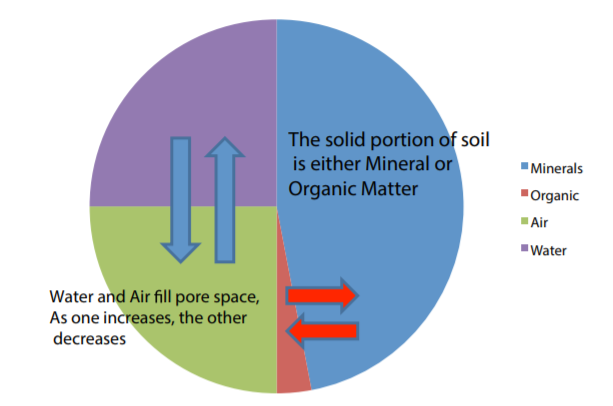
\includegraphics[height=60mm,width=100mm]{pie.PNG}
    \caption{Composition of Soil}
  \label{fig:Composition of Soil}
\end{figure}
\\.  
\pagebreak
\subsection{Basic properties of Soil}
Now let us discuss the key properties of soil that can be monitored or sensed
\subsubsection{Soil Texture}
Soil consists of 3 class of particles - silt, clay and sand. Their relative composition describes the texture of the soil. From the texture of the soil we mean that the coarse sand may feel gritty,
while a silt loam has the feel of
flour. \textit{\textbf{The composition of the soil is determined chemically by having the proper analysis of the fraction of clay, slit and sand. }}
\subsubsection{Soil Density and porosity}
The soil bulk density is defined as the ratio of mass of dry soil to the volume of the soil sample. Another density defined on soil is particle density which is the ratio of mass of dry soil to the volume of solid particles. In agricultural settings,
increasing bulk density indicates
compaction is occurring, which
could cause detrimental growing
conditions, such as limiting root
penetration or decreasing the soil
aeration process. \\
Soil porosity describes the portion
of the soil volume that can hold either air or water.
\subsubsection{Soil Water content}
The soil water content is the amount of water present in the soil pores. It is measured in percentages. Generally, we have following two type of measurement metrics available for the soil water content. \\
\[Gravimetric\, \% = \frac{(wet\,sample\,weight – dry\,sample\,weight) × 100}{dry\,sample\,weight} \]
\[Volumetric\, \% = \frac{(volume\,of\,water\,in\,sample) × 
100}{volume\,of\,soil\,sample} \]
The water sensors for the soil give their readings in the form of the volumetric percentages. Gravimetric methods are often avoided because they involve the process of drying the soil etc. 
\section{Available sensor technologies for Soil and Water}
In this section we will try to briefly discuss the various type of sensors available for the various different properties of the soil. Some of the properties are discussed in the previous sections. In the subsequent sections, we will discuss the principle behind the working of these sensors\footnote{Keeping the depth and the scope of this paper in mind, we will not be able to discuss the principles of all the instruments, but will try to give the brief idea about all of them.}.
\subsection{Soil Moisture sensor}
The soil moisture sensors detects the volumetric percentage of the moisture in the soil sample. They rely on the changes in the electrical properties of the soil such as dielectric constants of the sand, soil resistivity and the conductometric measurements. Soil moisture sensors typically refer to sensors that estimate volumetric water content. Following is one popular design of the soil moisture sensor\cite{ref2}

\begin{figure}[!h]
  %\includegraphics[scale = 0.75]{13.jpg}\\[0.0 cm]
  \centering
    \vspace*{0 cm}
  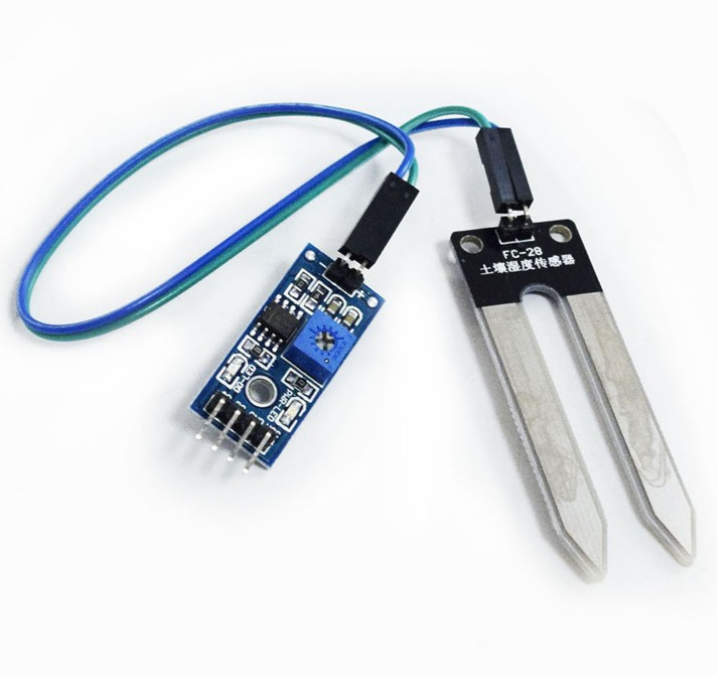
\includegraphics[height=80mm,width=100mm]{p1.PNG}
    \caption{Soil Moisture Sensor}
  \label{fig:Soil Moisture Sensor}
\end{figure}

\subsection{Water Potential Sensors}
Water potential is the potential energy of water per unit volume relative to pure water in reference conditions.Thus, water potential is related to the force that the plant need to apply to suck the water. Present techniques that calculate the water potential are \textbf{\textit{Tensiometers}} \cite{ref4}. This water potential determines the moisture distribution within the cell. \\ It consists of a shaft that contains water. This provides the connection between the soil water and the water inside the shaft. 
\textit{\textbf{Soil water potential is thus translated into a negative pressure inside the tensiometer that can be sensed by a mechanical gauge or electronic pressure sensor}}. Following is the structure of the tensiometer. Description of all parts are beyond the scope of this paper.

\begin{figure}[!h]
  %\includegraphics[scale = 0.75]{13.jpg}\\[0.0 cm]
  \centering
    \vspace*{0 cm}
  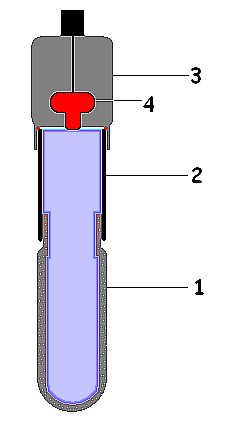
\includegraphics[height=80mm,width=80mm]{p2.png}
    \caption{Tensiometer}
  \label{fig:Soil Moisture Sensor}
\end{figure}
\subsection{Mechanical Sensors}
The mechanical sensors, as name suggests, they are used to determine the mechanical strength of the soil. Thus they play a very vital role in the crop development and to check the strength of the roots. Its probes go down in the ground and then records the resistive forces with the help of l\textbf{oad cells} or with the help of \textbf{strain gauges}. \textit{The strain gauges in the wheatsone connection will help in the measurement of strain.}
\subsection{Electrochemical Measurements}
For the crop to grow properly, its very important to maintain the ionic concentrations at the fixed level. The optimal pH for the proper growth of the plat is in the range 5.5 to 6.5. The electrochemical measurement based sensors deal with the measurements of these properties. This means, the pH, conductivity, ion activity and the concentration present inside the soil.\textit{\textbf{ They consists of glass electrodes from which we get the value of potential which with an ADC can be converted to digital values and can be transformed to suitable units of measurements. }}


\begin{figure}[!h]
  %\includegraphics[scale = 0.75]{13.jpg}\\[0.0 cm]
  \centering
    \vspace*{0 cm}
  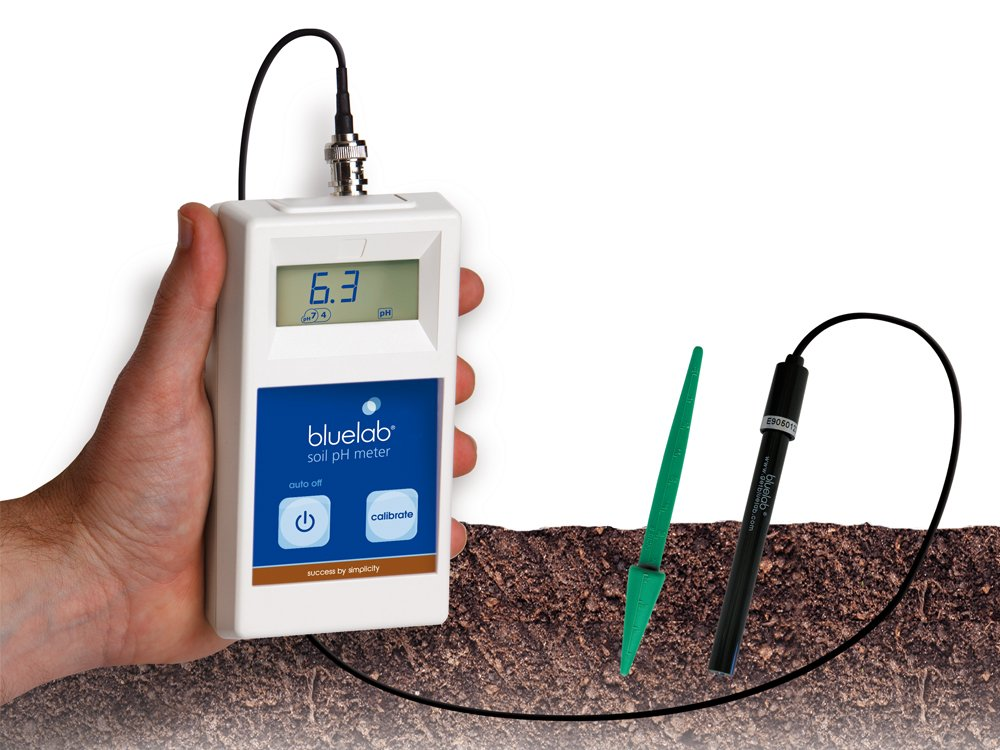
\includegraphics[height=80mm,width=100mm]{pp.jpg}
    \caption{Soil pH sensor}
  \label{fig:Soil Moisture Sensor}
\end{figure}

\subsection{Soil Temperature Sensors}
The temperature sensors employed in the soil are most basic RTD based sensors. They employ Pt100 sensor. Most of the temperature sensors work on the wide range of -30°C to +70 °C with 0 output at -30 °C and 3V output at +70°C. There are also temperature sensing ICs available with proper interfacing with the electronic micro controllers. For ex,\textbf{ \textit{we have SHT11 IC that can be connected with micro controller with an UART or I2C protocol.  }}
\begin{figure}[h]
  %\includegraphics[scale = 0.75]{13.jpg}\\[0.0 cm]
  \centering
    \vspace*{0 cm}
  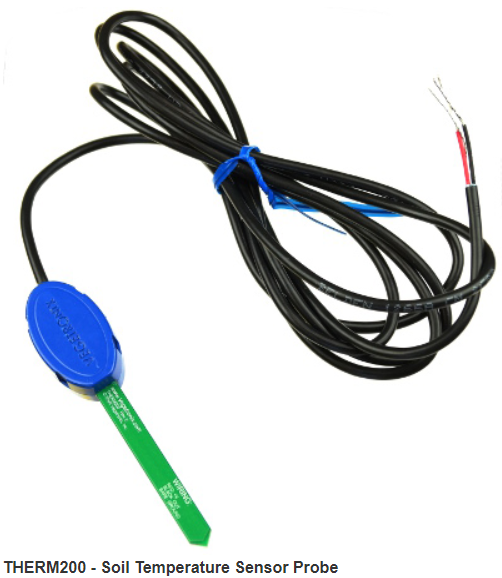
\includegraphics[height=60mm,width=60mm]{ppp.PNG}
    \caption{Soil temperature sensors}
  \label{fig:Soil Moisture Sensor}
\end{figure}
\pagebreak
\section{A Detailed Analysis of Moisture Sensors}
Moisture or the water content in the soil affects many of its physical (or mechanical) properties as well as its electrical properties. Most of the sensors built now exploit its electrical property. \textit{Other methods may involve the drying processes but the downside for that are they are very very slow method and won't give the real time measurement for the soil.\\}
Most of the electronic measurement devices, they work on the principle of change in some electrical parameter which they convert to the change in the voltage value .So, we need to calibrate the instrument with some reference value, and then depending upon the changes from that reference value it will give the results accordingly by taking care of the offsets.
\\
As mentioned earlier, the moisture sensors exploit the electrical properties. Following are some of the moisture sensors :- \\
\subsection{Capacitance Sensors}
The capacitance sensors exploit the change in the dielectric constant of the soil. The sensor has an oscillator. The shape of the moisture sensor is similar to a parallel plate capacitor system. When this sensor is inserted in the soil, the capacitance due to the soil dielectric changes the total capacitance of the system. Thus, this\textbf{ changes the natural frequency of the oscillator. The change in the oscillator frequency is detected by a phase lock loop}. Thus this phase lock loop which has a\textbf{ Voltage controlled oscillator converts this frequency to the voltage signal.} Hence now by processing the voltage signal, we can get the moisture content in the soil.

\subsection{Standing Wave Sensors}
This sensor uses the standing waves to determine the dielectric constant of the soil. In the soil, each water, air and the soil particles have different dielectric constants. Also, exploiting the fact that in a water:soil:air matrix, the dielectric constant is dominated by the amount of water present. Thus changes in the dielectric constant can be measured and hence we can measure the moisture content.
\subsection{TDT (Time Domain Transmissometry) Sensors}
These sensors emit an electromagnetic wave from one end of the probe to the other end through the soil medium. In the soil, because of the change in the dielectric constant, it will change the speed of the EM Wave, causing some delay in the form of phase\textit{.\textbf{ Thus, this delay manifested in the form of extra phase will now be recovered and then further processed to give the exact values of moisture content.}}
\pagebreak
\\
\textbf{
\emph{There are many other type of moisture sensor available but they are not feasible for the agriculture purpose. Some of them are Nuclear Magnetic Resonance technique based sensors, Gamma ray attenuation based sensors and Neutron scattering based sensors}.}

\section{Ion Concentration sensors}
Ionic concentration in the water is very important for the production of the crop. For their proper development they require a proper window of the ionic concentration. 

\begin{figure}[h]
  %\includegraphics[scale = 0.75]{13.jpg}\\[0.0 cm]
  \centering
    \vspace*{0 cm}
  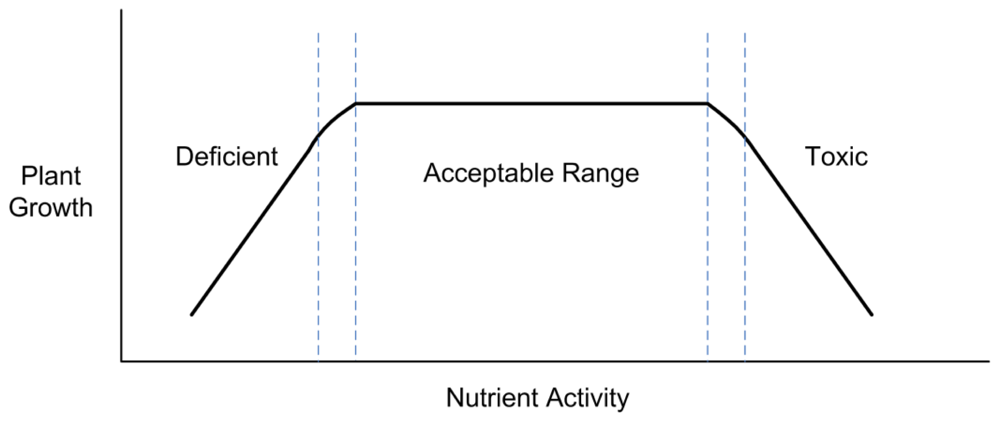
\includegraphics[height=60mm,width=100mm]{picc.png}
    \caption{Ionic Concentration graph for proper growth}
  \label{fig:Soil Moisture Sensor}
\end{figure}
In agriculture for the online measurements, we use pH meters and the conductivity meters to calculate the ionic concentrations. Here we will describe the working principle of these meters. The basic pH meter involve a chemical reaction at its electrodes. The chemical reaction governs the emf generated out of the electrode. It is mathematically formulated with the Nernst Equation.\\
\textit{The Nernst Equation enables the determination of cell potential under non-standard conditions. It relates the measured cell potential to the ratio of the concentrations. It is formulated as -}
\begin{equation} \label{eq:1}
E = E_0 - \frac{RT ln(Q)}{nF}
\end{equation}
where F is the farady constant, n is the electrons exchanged in the reaction, Q is the ratio of concentrations and \(E_0\) is the standard cell potential. Thus, now we can explain the working of pH meters. \\
\begin{description}
\item[$\ast$] pH meters calculate the voltages developed due to the ratio of concentration at the electrodes. 
\item[$\ast$]If the soil water or the water has more ionic concentration or more \(H^{+}\) then more will be the current flowing through the water.  
\item[$\ast$] In order to current to flow, the circuit has to be completed. This circuit is completed by the conducting water in the soil. The sample soil comes into contact with two electrodes which are found on the probe.
\item[$\ast$] pH meters have two electrodes, a glass electrode and a reference electrode.
The glass electrode has a permeable membrane made from specialised glass, which houses a chemical solution and a silver-based wire. The reference electrode is also made up of a wire in a chemical solution. 
\item[$\ast$] The reference electrode act as a buffer and with respect to this electrode due to the concentration difference of H ions, as per the Nernst Equation (\ref{eq:1}) we get a DC voltage appearing across the terminals. 
\item[$\ast$] This voltage difference is sent to the signal processing chip, that converts it to the pH value. 
\end{description}


\begin{figure}[h]
  %\includegraphics[scale = 0.75]{13.jpg}\\[0.0 cm]
  \centering
    \vspace*{0 cm}
  \includegraphics[height=50mm,width=140mm]{lol.png}
    \caption{Glass Electrode \cite{ref4}}
  \label{fig:Soil Moisture Sensor}
\end{figure}

\section{Towards the robustness and online monitoring of sensors}
So far we have discussed about different kind of sensors and have discussed 2 sensors in detail which were about the Moisture sensor and the pH sensor. In this section, we will discuss about some of their advantages, their robustness and places where they fails. \\
\subsection{Moisture Sensor}
Here we will discuss some advantages, methods for online monitoring and some disadvantages.\\
\subsubsection{Data storage and Transmission}
\begin{itemize}
    \item They can be easily connected to the DC loggers. Since we use Voltage controlled oscillators to determine the value of frequency of the oscillations in the form of voltages, they can be stored easily.
    \item We can use arduino to store the values and can link it with WiFi. With the help of wifi, to avoid the transient measurements, we can send every 10 readings to the master controller. Where it can be further decoded to see the values.
\end{itemize}
\subsubsection{A 2 step controller design to automate watering}
We can use our sensors to design a two step controller for the watering. By setting up the upper and the lower bound of the desired moisture contents we can make a controller that turns on the water supply if the level falls off the lower bound, and can have some drying mechanism if the level go beyond the certain level. \\
Though, we know that for a proper control which do not involve much oscillations, a continuous control is a better choice, but here keeping the feasibility and the operational cost in mind, 2 step controller is a good idea.
\\
\subsubsection{Some disadvantages for the sensors}
Following are some of the disadvantages where these sensor fails: - \\
\begin{itemize}
    \item The capacitance sensors have much smaller area. Thus we will need to buy a lot of them to have a correct monitoring. 
    \item Capacitance sensors are highly sensitive towards the temperature. Thus, we cannot have much accurate measurements if the temperature fluctuates. Though we can use a temperature sensing IC along with this and have a complex circuit that involve implementation of the mathematical relation between the T and C, but that will increase the cost. Hence not feasible as far as poor farmers are concerned. 
    \item For the TDT (Time Domain Transmissometry) Sensors, their precision is reduced because of the distortion of the generated pulse while the transmission.
\end{itemize}

\subsection{pH Sensors}
As we had discussed that the pH sensors converts the voltage developed across the electrodes to the pH values, we can save the values of the pH and with the help of arduino and WIFI interface, we can transmit the data to the master control center so that one don't have to move inside the fields to manually monitor the readings.

\subsubsection{Some disadvantages for the pH sensors}
\begin{itemize}
    \item The pH highly depends on the buffer solutions filled inside the reference electrodes. Thus one has to take proper care of the reference electrode and need to check its quality time to time.
    \item The generated voltage across the terminals of the electrode is temperature dependent. Thus during the measurement if there are changes in the temperatures, then one can have faulty readings. 
    \item As we have the additional temperature measurement ICs along with the pH measurement, the cost of the complete system increases. Thus for the Indian Agriculture setting these automated electronic measuring instruments cost heavily on the pockets.
\end{itemize}
\section{Concluding Remarks}
Thus in this paper we studied about different properties of soil and surveyed many different available sensors. Later we studied about there robustness and also provided a simple but efficient way to automate the watering in the fields. Due to the limited scope of this paper, we didn't discuss about the economic aspects of these sensors. Any product that we are designing should be easily accessible to the farmers both in terms of money as well as in terms of handling. As future work we can discuss about the conventional farming techniques and bio monitoring with biological sensors such as earthworm etc. and then try to improve them with the science and technology.

\begin{thebibliography}{9}
\bibitem{ref1}
Irrigation management series\\
\texttt{https://www.ksre.k-state.edu/irrigate/reports/r15/L935.pdf}
\bibitem{ref2}
Soil Moisture Sensors
\texttt{https://www.smart-prototyping.com/Soil-Hygrometer-Detection-\\Module-Soil-Moisture-Sensor-For-Arduino.html}
\bibitem{ref3}
pH meter \\
\texttt{https://hannainst.in/}
\bibitem{ref4}
Glass Electrodes
\texttt{https://www.wonkeedonkeetools.co.uk/media/wysiwyg\\/18SPM-Soil-PH-Meter-Jenna/18SPM07/18SpM_7-5.jpg}

\bibitem{ref5}
Electronic Tensiometers
\texttt{https://www.agroengineering.org/index.php/jae/article\\/view/jae.2013.e16/459#figures}
\bibitem{ref6}
Fedro S. Zazueta and Jiannong Xin2, Soil Moisture Sensors, University of Florida
\bibitem{ref7}
Datasheet SHT1x
\texttt{https://www.sparkfun.com/datasheets/Sensors/SHT1x_datasheet.pdf}

\end{thebibliography}


\end{document}